\section{Importancia del ancho de banda en la performance}
El ancho de banda de la conexión es un factor importante al analizar la performance en una aplicación web, sin embargo, el \emph{round-trip-time} tiene una influencia aún mayor en la performance de las páginas web. El \emph{round-trip-time} o RTT es el tiempo que tarda un paquete enviado por un emisor en llegar al receptor más el tiempo que tarda en llegarle un mensaje de confirmación de recepción por parte del receptor. Debido a que las páginas web están compuestas por varios objetos se utilizan varias conexiones TCP diferentes cortas que no logran utilizar todo el ancho de banda disponible como lo harían
las descargas de grandes contenidos como videos, audio, etc.

\subsection{Ancho de banda y RTT}
Mientras que aumentar el ancho de banda puede resultar relativamente sencillo, minimizar el RTT es una tarea compleja, debido a que el tiempo que tarda un paquete está limitado
entre otros factores por la velocidad de la luz. Los paquetes enviados viajan a través de fibra que está compuesta por materiales que ofrecen cierta resistencia, generando una disminución de la velocidad de transmisión en un factor de aproximadamente 1.52.
En caso de que un servidor se encuentre en Londres y el cliente en San Francisco, el tiempo que tardaría la luz en recorrer esa distancia sería aproximadamente 30ms, y en el caso de un RTT 60ms ya que se debe recorrer la distancia dos veces, una cuando se envía el paquete y la segunda cuando se envía el paquete de confirmación en sentido contrario.
En la actualidad, los RTT en internet rondan entre los 150ms y 250ms, independientemente del ancho de banda que se tenga.

Los siguientes resultados están basados en el trabajo realizado por Mike Belshe en \cite{mike_belshe}  y el
artículo escrito por Ilia Grivorik \cite{grivorik}, en los cuales se realiza un estudio de como las distintas 
variaciones del ancho de banda y el RTT afectan los tiempos de respuesta de las aplicaciones web.

\subsection{Variación del ancho de banda}
El primer análisis que realizaron fue el estudio de los efectos que tiene la variación del ancho de banda de la red en los tiempos de descarga de una página web.
Tomaron medidas para aislar la variable que estaban estudiando (en este caso el ancho de banda), fijando valores para la pérdida de paquetes (0\%) y el RTT en 60ms.
A continuación se muestran los resultados del mismo.

\begin{figure}[h!]
\centering
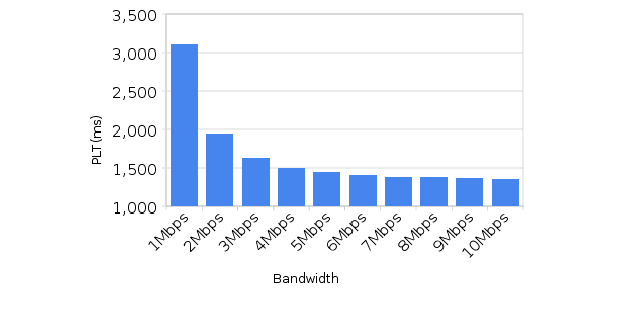
\includegraphics[width=1\textwidth]{figuras/latencyperbandwidth.png}
	\caption{Latencia per Bandwidth}
    \label{fig.latency-per-bandwidth}
\end{figure}

En la figura \ref{fig.latency-per-bandwidth} se puede observar como disminuye la latencia a medida que aumenta el ancho de banda. Sin embargo, observamos también que dicha tendencia tiende a disminuir a partir de los 5Mbps de ancho de banda.
Según el reporte del estado de internet de Akamai del año 2011 \cite{akamai} el consumidor promedio de internet en los Estados Unidos cuenta con un ancho de banda mayor a los 5Mbps, por lo cual la mayoría de los usuarios de Estados Unidos no obtendría un gran beneficio al aumentar su ancho de banda.

\begin{figure}[h!]
\centering
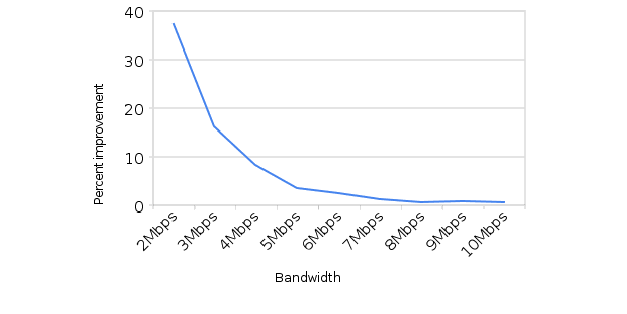
\includegraphics[width=1\textwidth]{figuras/beneficiodembpsextras.png}
	\caption{Beneficio de agregar Mbps extras}
    \label{fig.beneficioextrambps}
\end{figure}

En la \ref{fig.beneficioextrambps} se puede apreciar como disminuye la mejora en porcentaje de la latencia a medida que se aumenta el ancho de banda. Como se puede apreciar,
un incremento de un 100\% en el ancho de banda (de 5Mbps a 10Mbps), genera una mejora en el tiempo de carga de una página de solamente un 5\%.

\subsection{Variación del RTT}
Las condiciones para estos casos de prueba consistieron en mantener constante el ancho de banda durante todo el experimento en 5Mbps y variar el RTT de 0ms a 240ms.

\begin{figure}[h!]
\centering
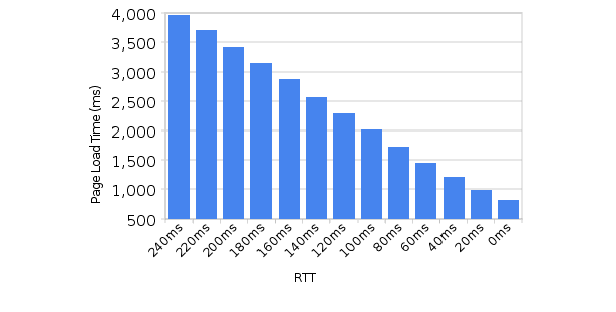
\includegraphics[width=1\textwidth]{figuras/page_load_time_as_rtt_decreases.png}
	\caption{Variación en el tiempo de carga de una página a medida que el RTT disminuye}
    \label{fig.pageloadtimeasrttdecreases}
\end{figure}

Como se puede apreciar en la figura \ref{fig.pageloadtimeasrttdecreases}, existe una relación directa entre el tiempo de carga de una página y
la duración del RTT. A medida que el RTT disminuye también lo hace el tiempo de carga.

\begin{figure}[h!]
\centering
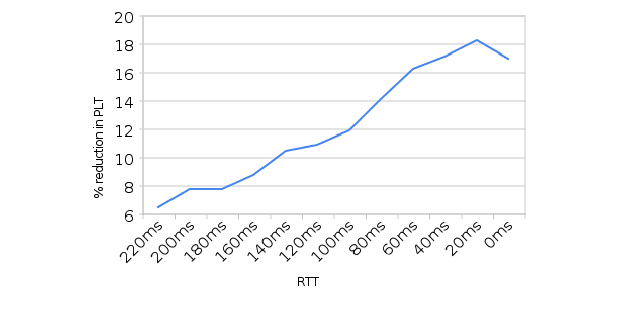
\includegraphics[width=1\textwidth]{figuras/beneficios_de_disminuir_rtt.png}
	\caption{Beneficio de reducir el RTT}
    \label{fig.beneficiosdedisminuirrtt}
\end{figure}

En la figura \ref{fig.beneficiosdedisminuirrtt} se muestra el porcentaje de reducción del tiempo de carga de una página por cada 20ms de reducción del RTT.

\subsection{Conclusión}

En base a los datos obtenidos en los experimentos se puede concluir que si un usuario duplica su ancho de banda sin reducir en forma significativa el RTT, la mejora
que percibirá el usuario en la navegación por la web no será muy notoria. Por otro lado, disminuir el RTT sin importar el ancho de banda que se tenga siempre beneficia
la navegación.

Un enfoque a tomar al momento de reducir el tiempo de carga de una página debería ser reducir la cantidad de RTTs necesaria para que la página cargue. El elevado número
de \emph{round trips} se debe en parte a los intercambios de paquetes necesarios para iniciar la comunicación entre el cliente y el servidor (por ejemplo DNS, TCP, HTTP),
y a su vez por \emph{round trips} introducidos por los protocolos de la capa de transporte como TCP, el cual sufre del fenómeno denominado \emph{slow start}.

